\documentclass[HeilHazel,pdf,final,colorBG,slideColor]{prosper}
\usepackage{tikz}
\usepackage{epsfig}
\usepackage{amsbsy,amsmath}
\usepackage{rotating}
\usepackage{graphicx}
\usepackage{color}
\usepackage{amsbsy}
\usepackage{epsfig}
\usepackage{natbib}
\usepackage[a6paper,centering]{geometry} % Utilise pour centrer

\usepackage[francais]{babel}

\NoFrenchBabelItemize
\usepackage{ucs}
\usepackage[utf8x]{inputenc}
% \usepackage{graphicx,color,caption2,amssymb,pstricks,lmodern}

\setlength{\unitlength}{1cm}
\NoFrenchBabelItemize



\title{\vspace{-0,5cm}Senior capstone project, MSc Alma}
\subtitle{Soutenance de projet}
\author{N.\textsc{Boukra}, L.\textsc{Duringer}\\
  A.\textsc{Marguerite},  M.\textsc{Ouairy}\\
  \& N.\textsc{Sebari}}
\institution{\vspace{0.5cm} {\hspace{1cm}
\includegraphics[scale=0.13]{img/logouniv} \hspace{.5cm}
\includegraphics[scale=0.2]{img/logoobeo} }  \vspace{0.3cm}\\  University of Nantes }
%\email{}
%\slideCaption{Université de Nantes, FR 
\includegraphics[scale=0.05]{img/logouniv}}
%\Logo{
\includegraphics[scale=0.05]{img/logouniv}}
\DefaultTransition{Dissolve}


\begin{document}

\maketitle
\newcommand{\bc}{\begin{center}} 
\newcommand{\ec}{\end{center}} 
\newcommand{\bi}{\begin{Itemize}} 
\newcommand{\ei}{\end{Itemize}} 
\newcommand{\myitemm}{\item \includegraphics[width=.4cm]{green-bullet-on-white}}
\myitem{1}{\includegraphics[width=.4cm]{red-bullet-on-white}}
%\myitemm{2}{\includegraphics[width=.4cm]{green-bullet-on-white}}
\newcommand{\icongb}{\includegraphics[width=.4cm]{green-bullet-on-white}} 
\newcommand{\iconrb}{\includegraphics[width=.4cm]{red-bullet-on-white}} 

\newcommand{\itemg}{\item[\icongb{}]}
\newcommand{\itemr}{\item[\iconrb{}]}


\begin{slide}{Sommaire}
  \begin{enumerate}
    {\bf
    \item L'entreprise Obeo
      \vspace{.5cm}
    \item Objectifs \& démarches
      \vspace{.5cm}
    \item Technologie cible  
      \vspace{.5cm}
    \item Contribution
      \vspace{.5cm}
    \item Conclusion}
  \end{enumerate}
\end{slide}


\overlays{3}{%
  \begin{slide}{L'Entreprise Obeo}
    \vspace{-1cm}
    \begin{itemstep}
      \fromSlide{1}{\itemg Concepteur de solutions logicielles}
      \vspace{1cm}
      \fromSlide{2}{\itemg À l'origine du projet \textit{Acceleo}\\ \hspace{4cm} 
\includegraphics[scale=.20]{img/logoacceleo.eps}}
      \vspace{1cm}
      \fromSlide{3}{\itemg Membre stratégique de la \textit{fondation Eclipse} \\ \hspace{4cm}  
\includegraphics[scale=.45]{img/logoeclipse.eps}}
    \end{itemstep}
  \end{slide}
}

% CONTEXTE (liste relatant les notions abordées ?)
\overlays{3}{%
  \begin{slide}{Contexte}
  
    \begin{itemstep}
    \itemg Des générateurs de code pour le web existent ...
    \itemg ... mais ces générateurs génèrent du code bas niveau, difficilement maintenable
    \itemg De nombreux framework web existent
    \end{itemstep}
  
  \end{slide}
}

% OBJECTIFS (liste aussi (conception modèle, générateur) ?)
\overlays{5}{%
  \begin{slide}{Objectifs}

    \begin{itemstep}
    \itemg Analyser les framework Web existants
    \itemg Étudier leur compatibilité avec la démarche de génération de code
    \itemg Choisir un framework adapté, et courament utilisé
    \itemg Réaliser un générateur de code pour la technologie choisie
    \end{itemstep}
    \bc{}
    \fromSlide{5}{
\includegraphics[scale=.4]{img/logoPlay.eps} }
    \ec{}
  \end{slide}
}

% ORGANISATION (dur d'en faire une diapo, mais neamoins tres important)
% (je laisse en liste/overlays en attendant)
\overlays{1}{%
  \begin{slide}{Organisation}
  \bc{} 
  \centering
    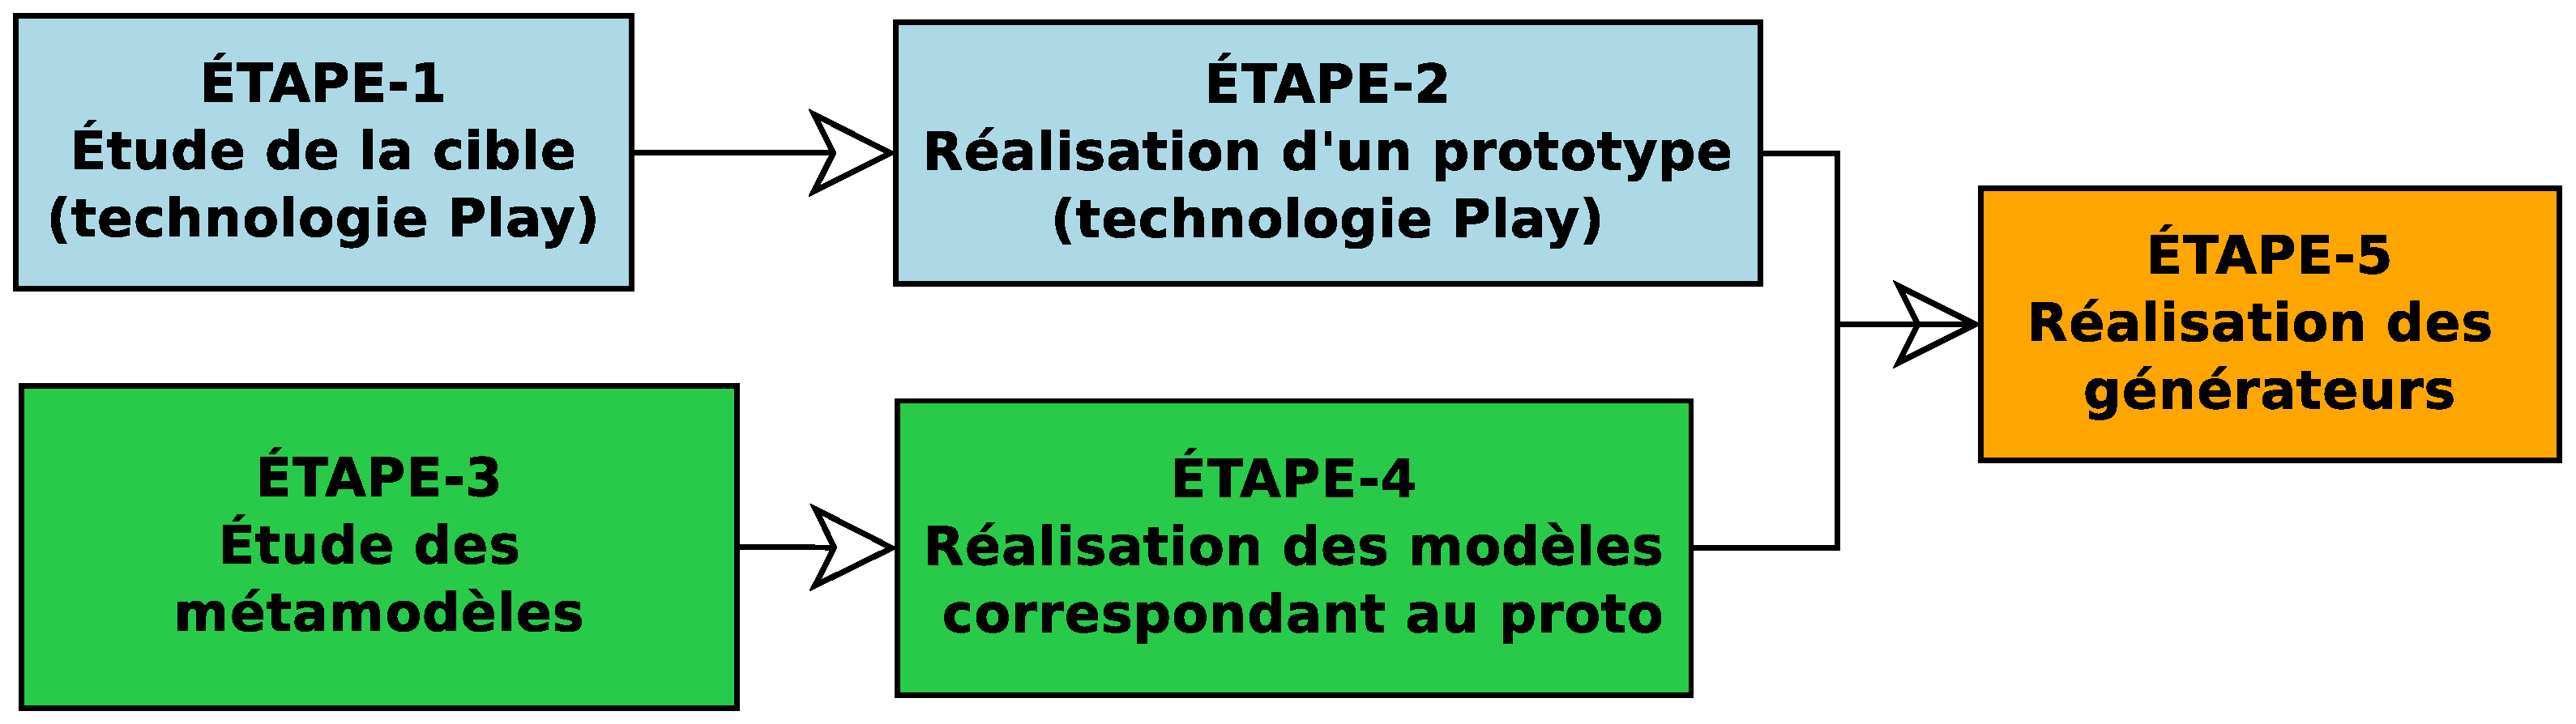
\includegraphics[scale=.22]{img/demarche.eps} 
  \ec{}
  \end{slide}
}


% Presentation Play
\begin{slide}[Box]{Le Framework \textit{Play!}}
\bigskip
  \begin{center}
  \centering
    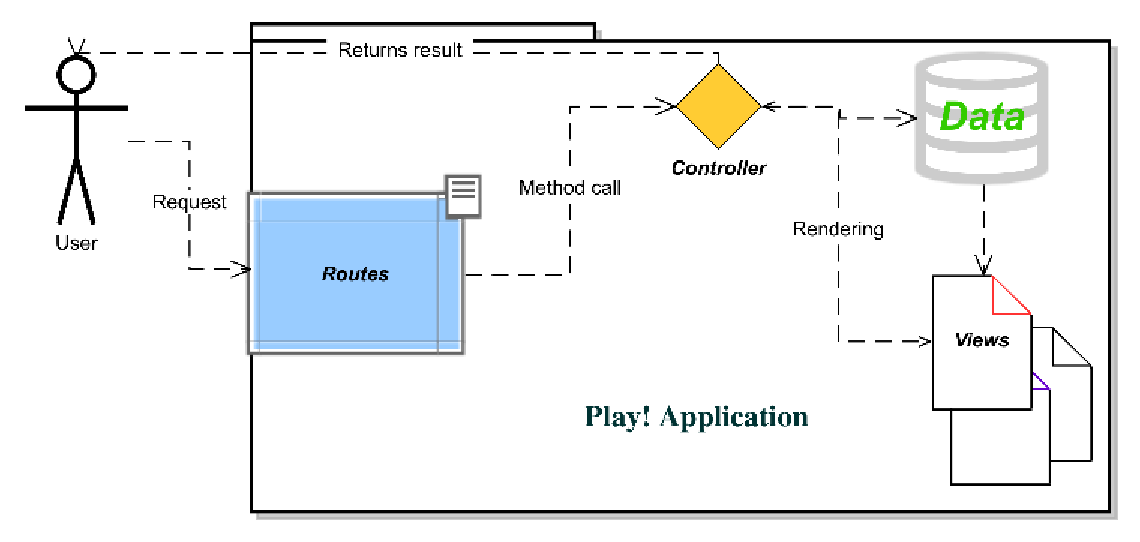
\includegraphics[scale=.6]{img/play_scheme.eps} 
  \end{center}
\end{slide}

% Prototype d'application avec screen
\begin{slide}[Box]{Prototype d'application}
  %\vspace{-1cm}
  \bc{} 
    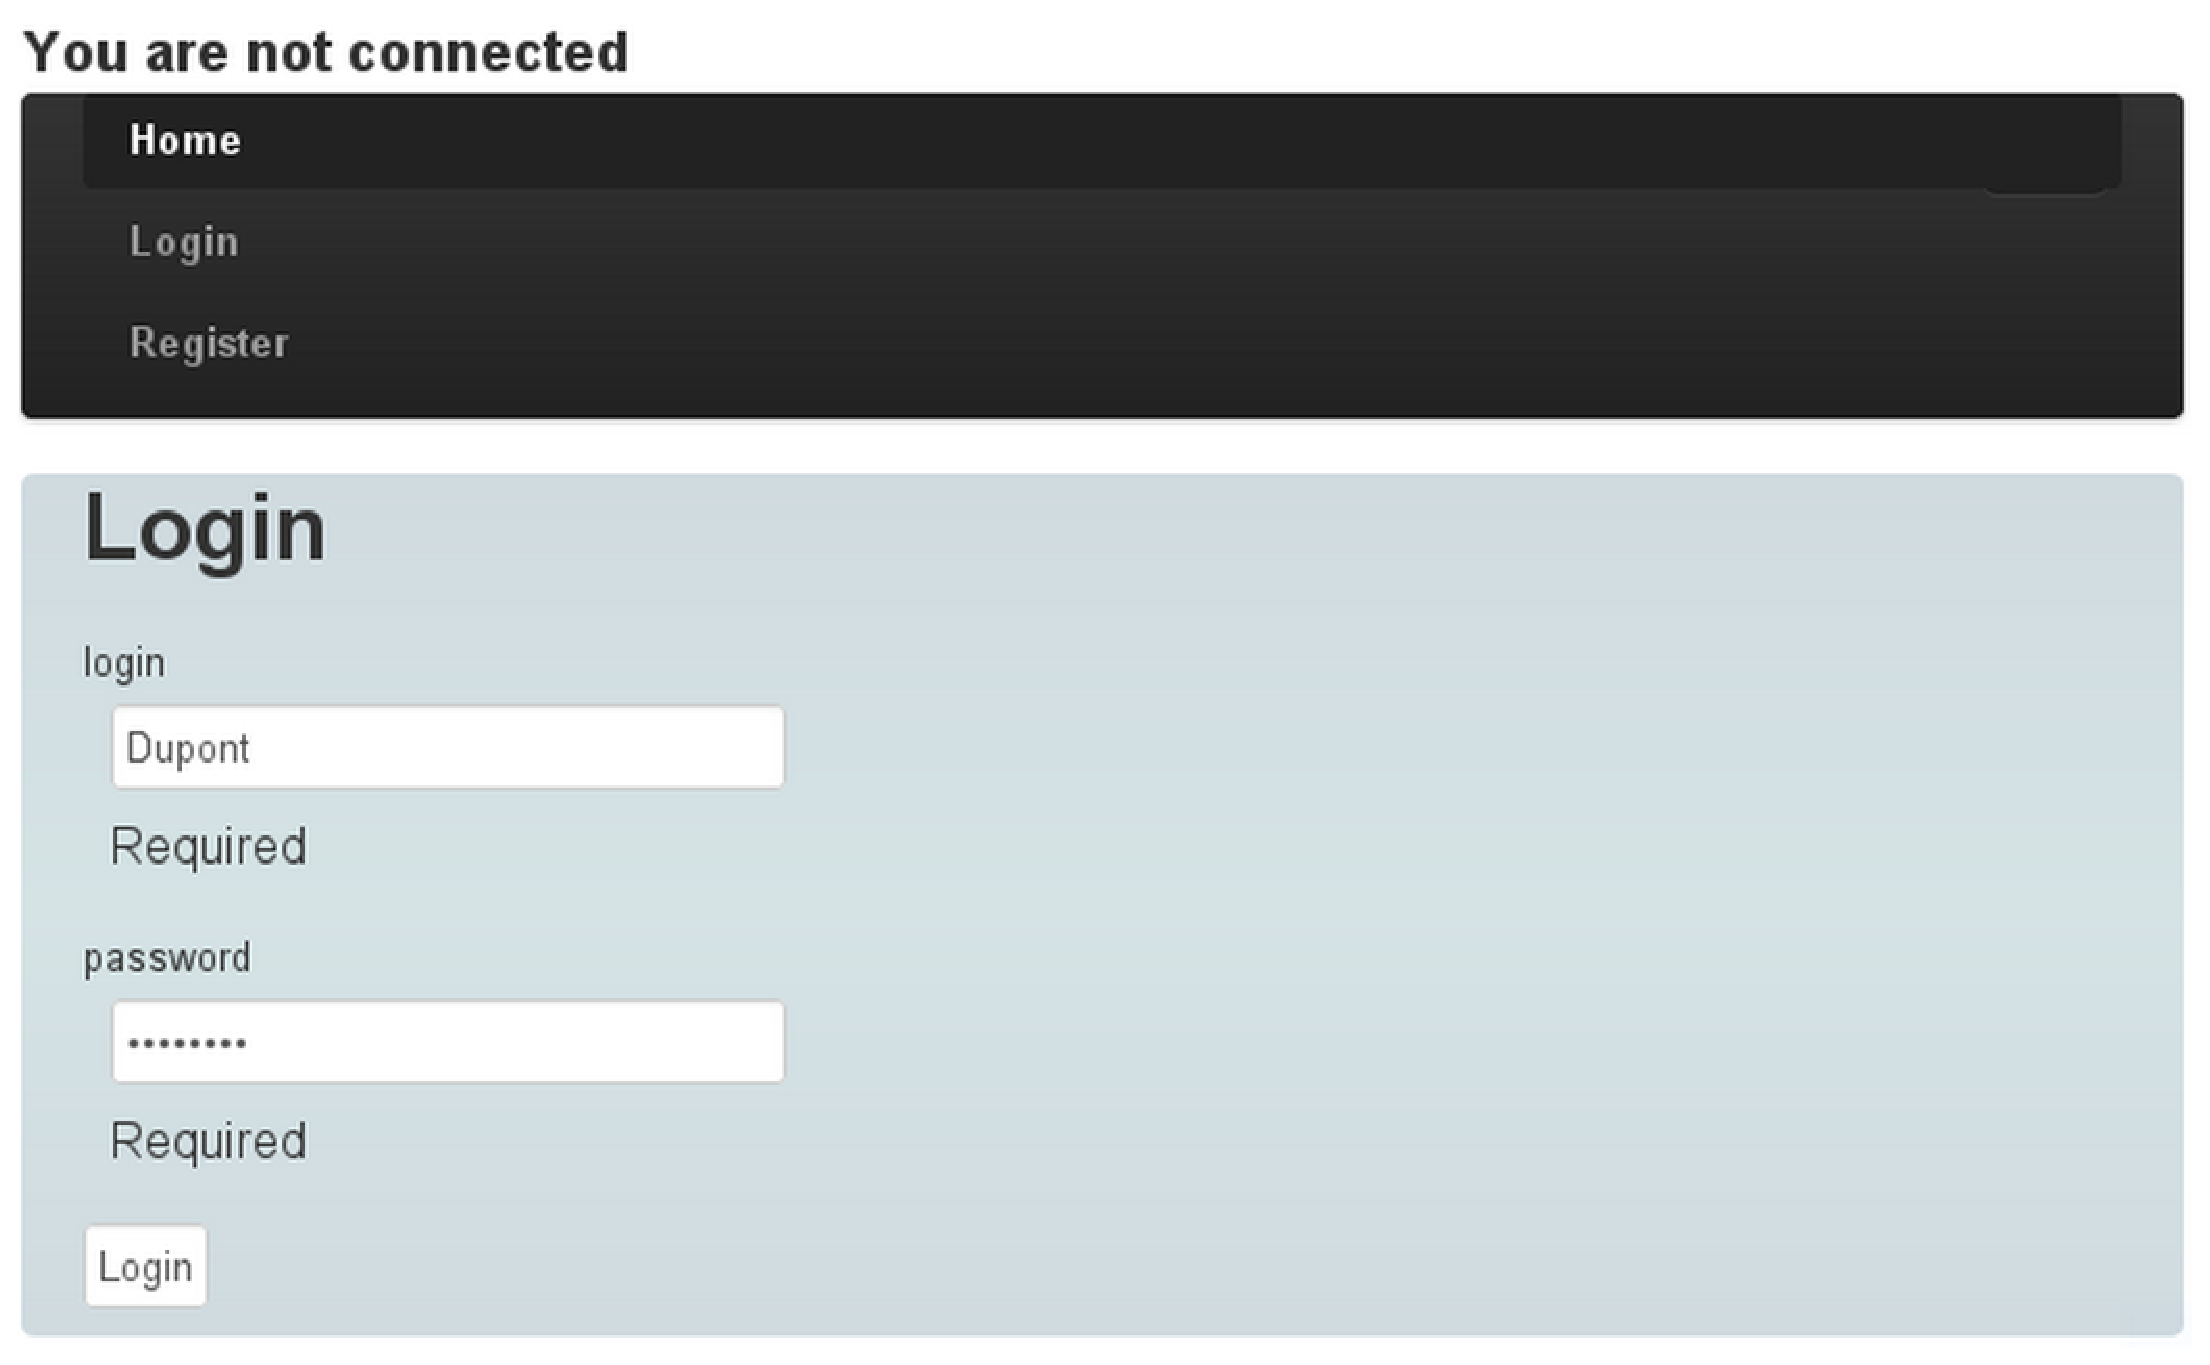
\includegraphics[scale=.3]{img/screen_prototype.eps} 
  \ec{}
\end{slide}

% TRAVAUX 
\overlays{3}{%
  \begin{slide}{Travaux}
  
    \begin{itemstep}
    \itemg Conception de 3 Modèles.
    \itemg Conception de 3 générateurs.
    \itemg Application principale
    \end{itemstep}
  
  \end{slide}
}

\begin{slide}{Travaux > Entity}


\end{slide}


\begin{slide}{Travaux > Entity}

\end{slide}


% SOA : M2 simple
\begin{slide}{Travaux > SOA}

  \bc{} 
    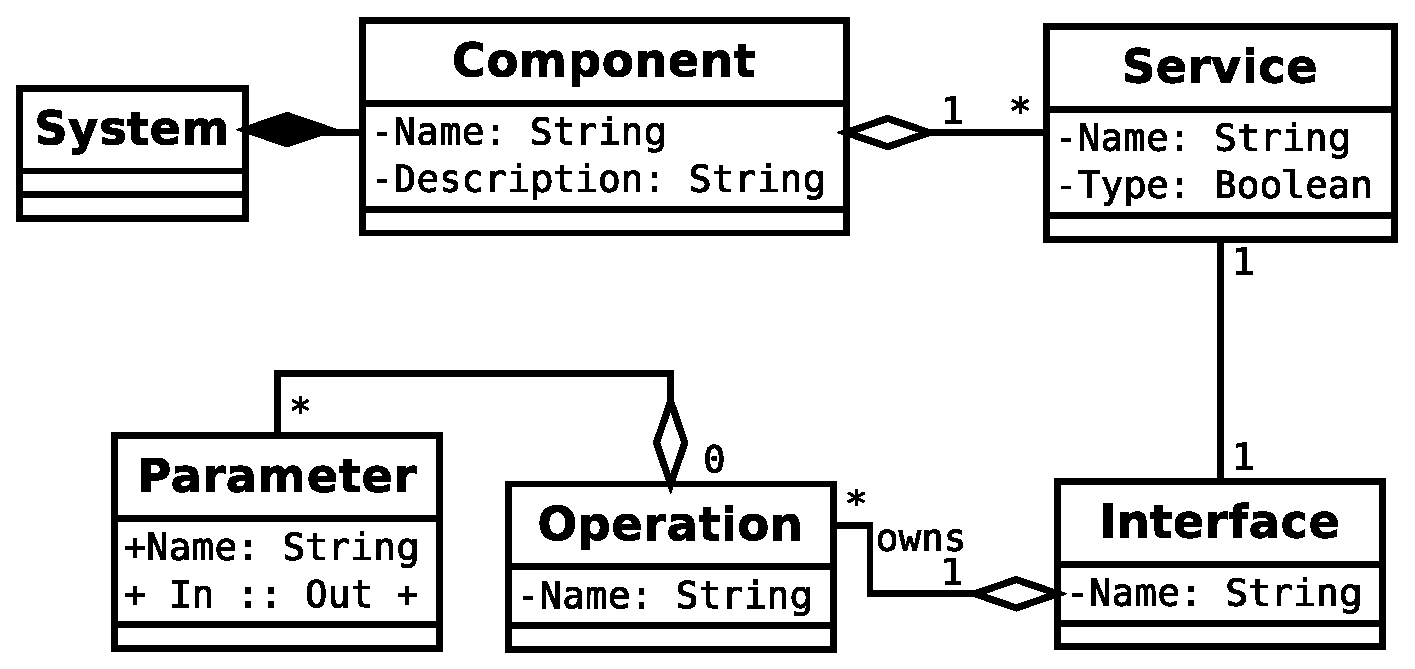
\includegraphics[scale=.45]{img/SOA_simple.eps}
  \ec{}

\end{slide}

% SOA : Implementation
\begin{slide}{Travaux > SOA > Mise en place}

  \bc{} 
    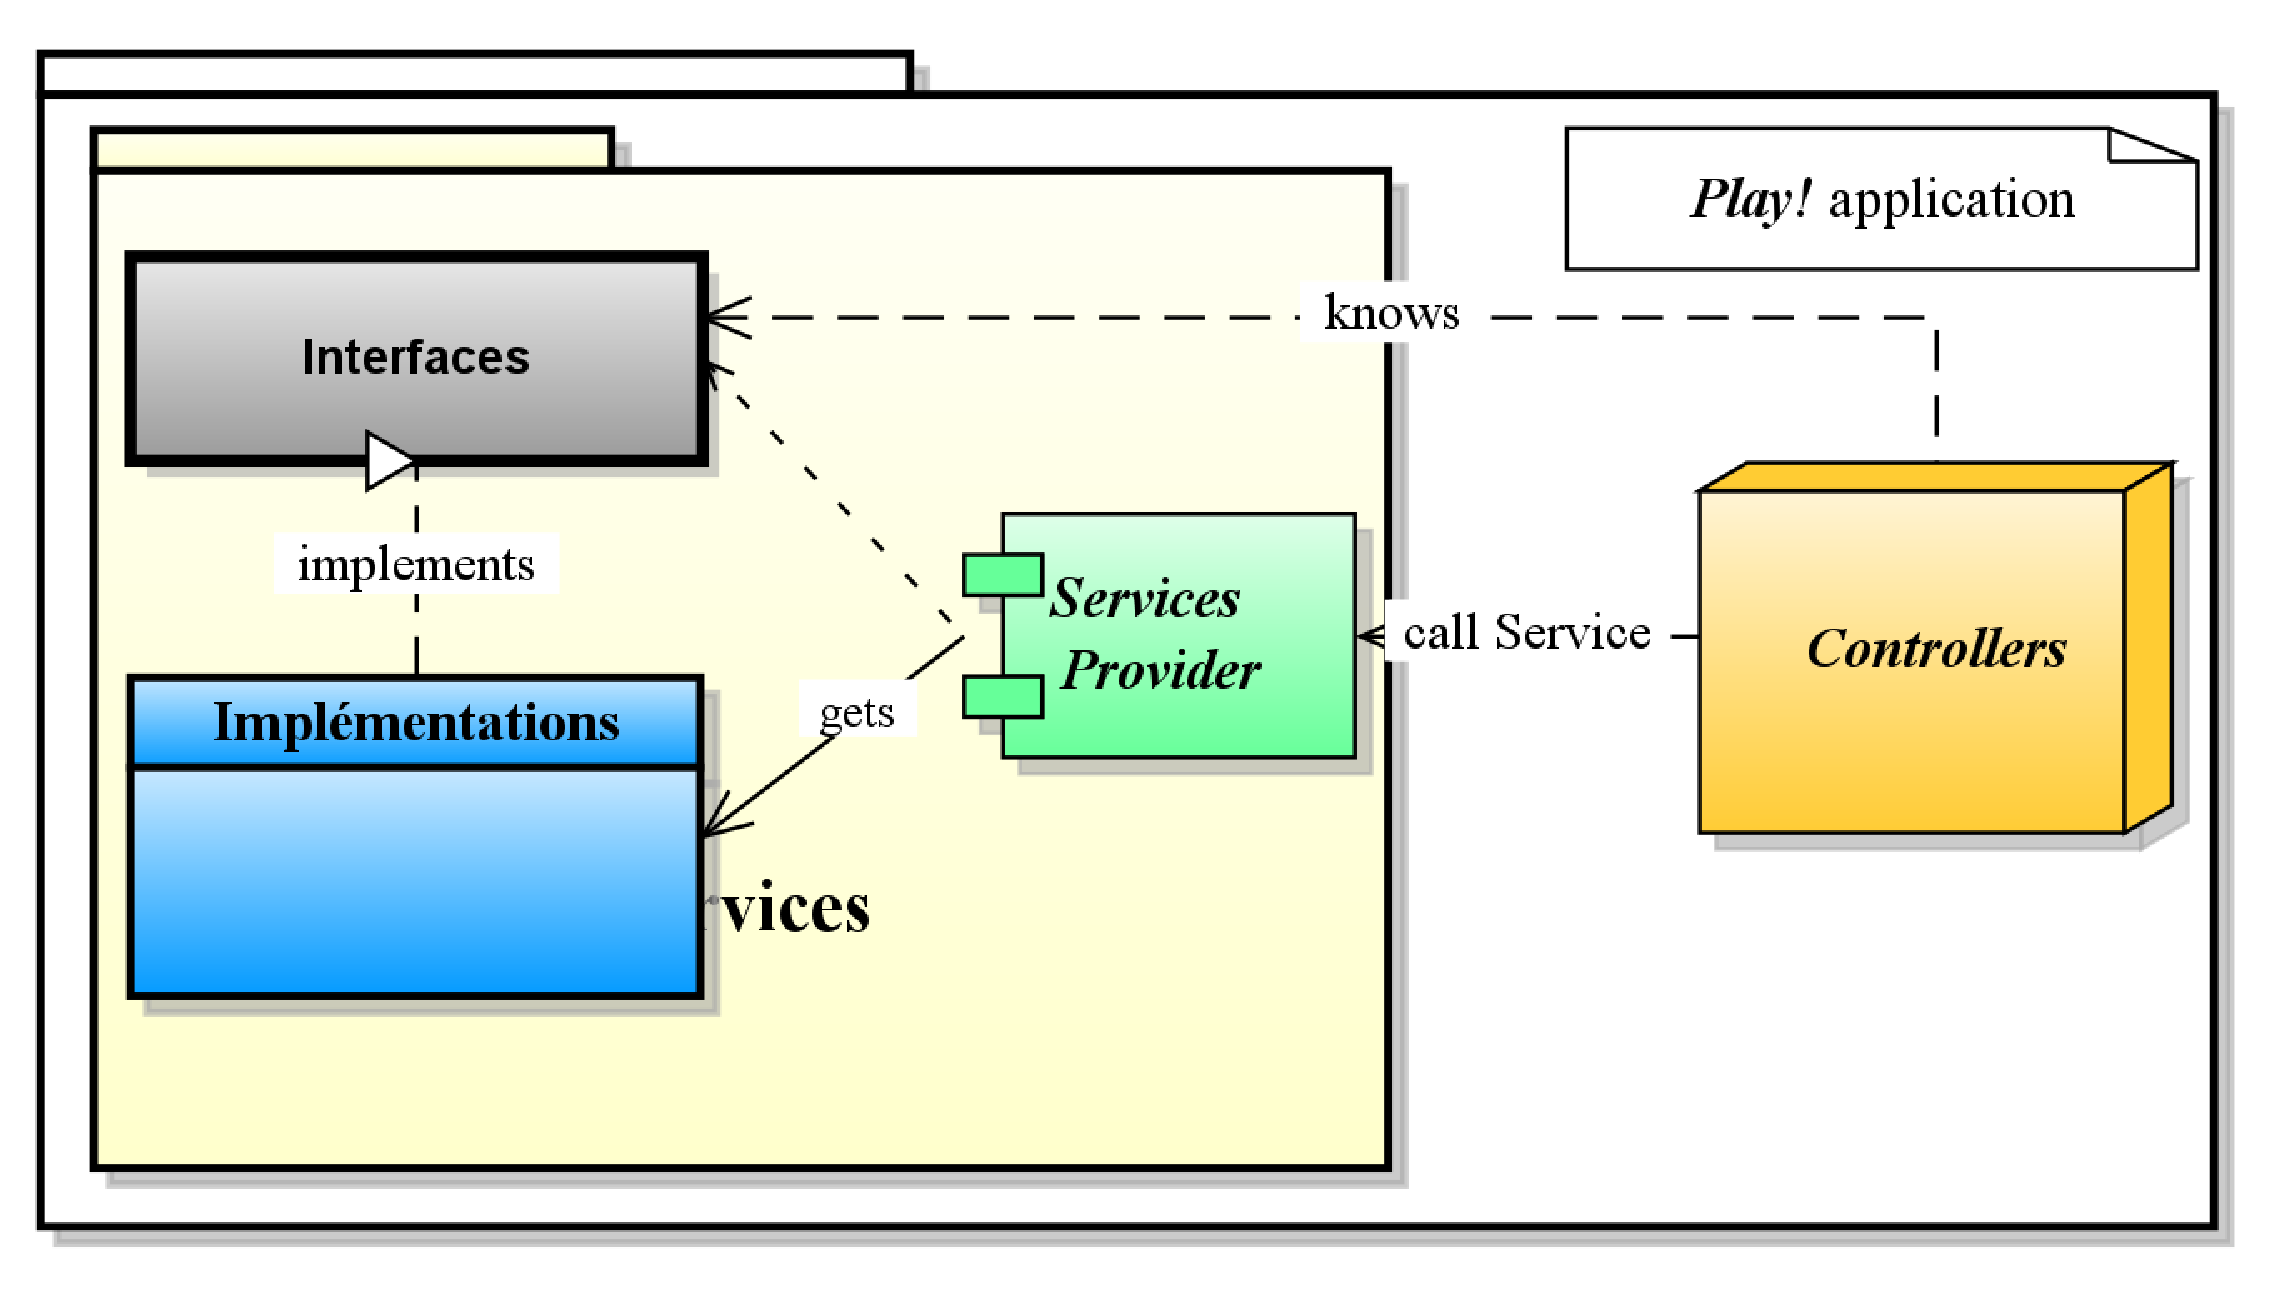
\includegraphics[scale=.3]{img/SOA_impl.eps} 
  \ec{}

\end{slide}

% SOA : Webservices
\begin{slide}{Travaux > SOA > Webservices}

  \bc{} 
    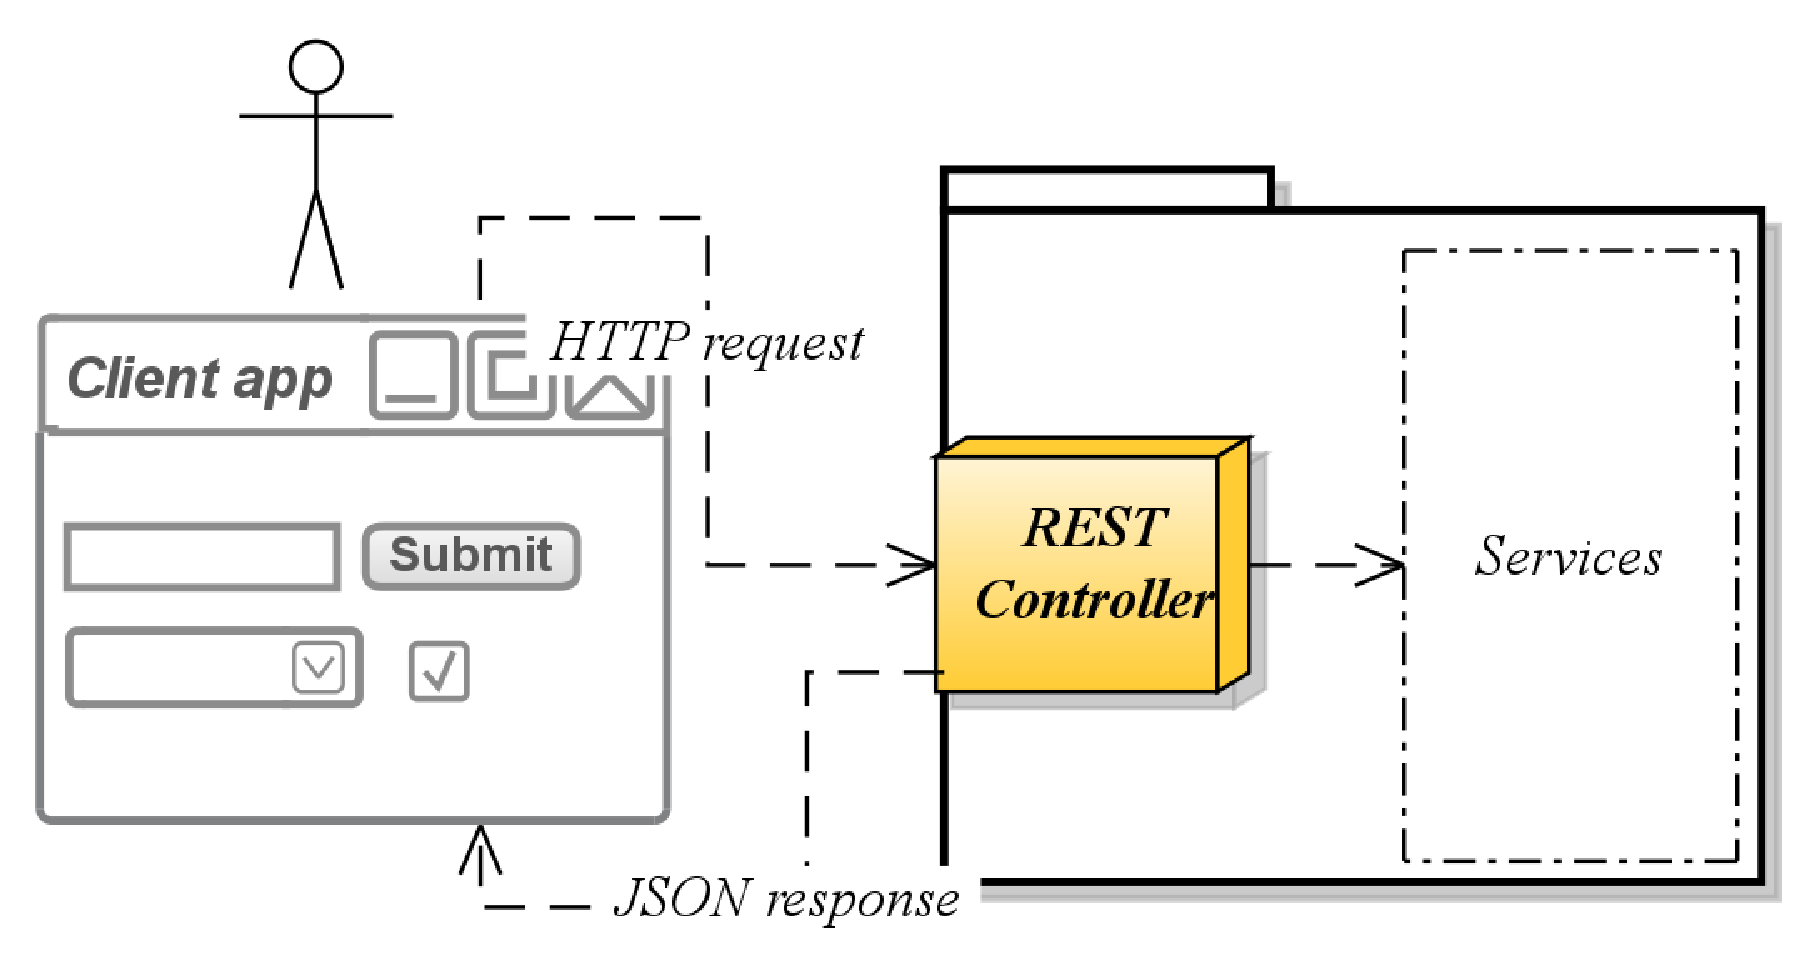
\includegraphics[scale=.4]{img/SOA_WS.eps} 
  \ec{}

\end{slide}

% Cinematic : Le M2
\begin{slide}{Travaux > Cinematic > Méta-Modèle}

  \bc{}
    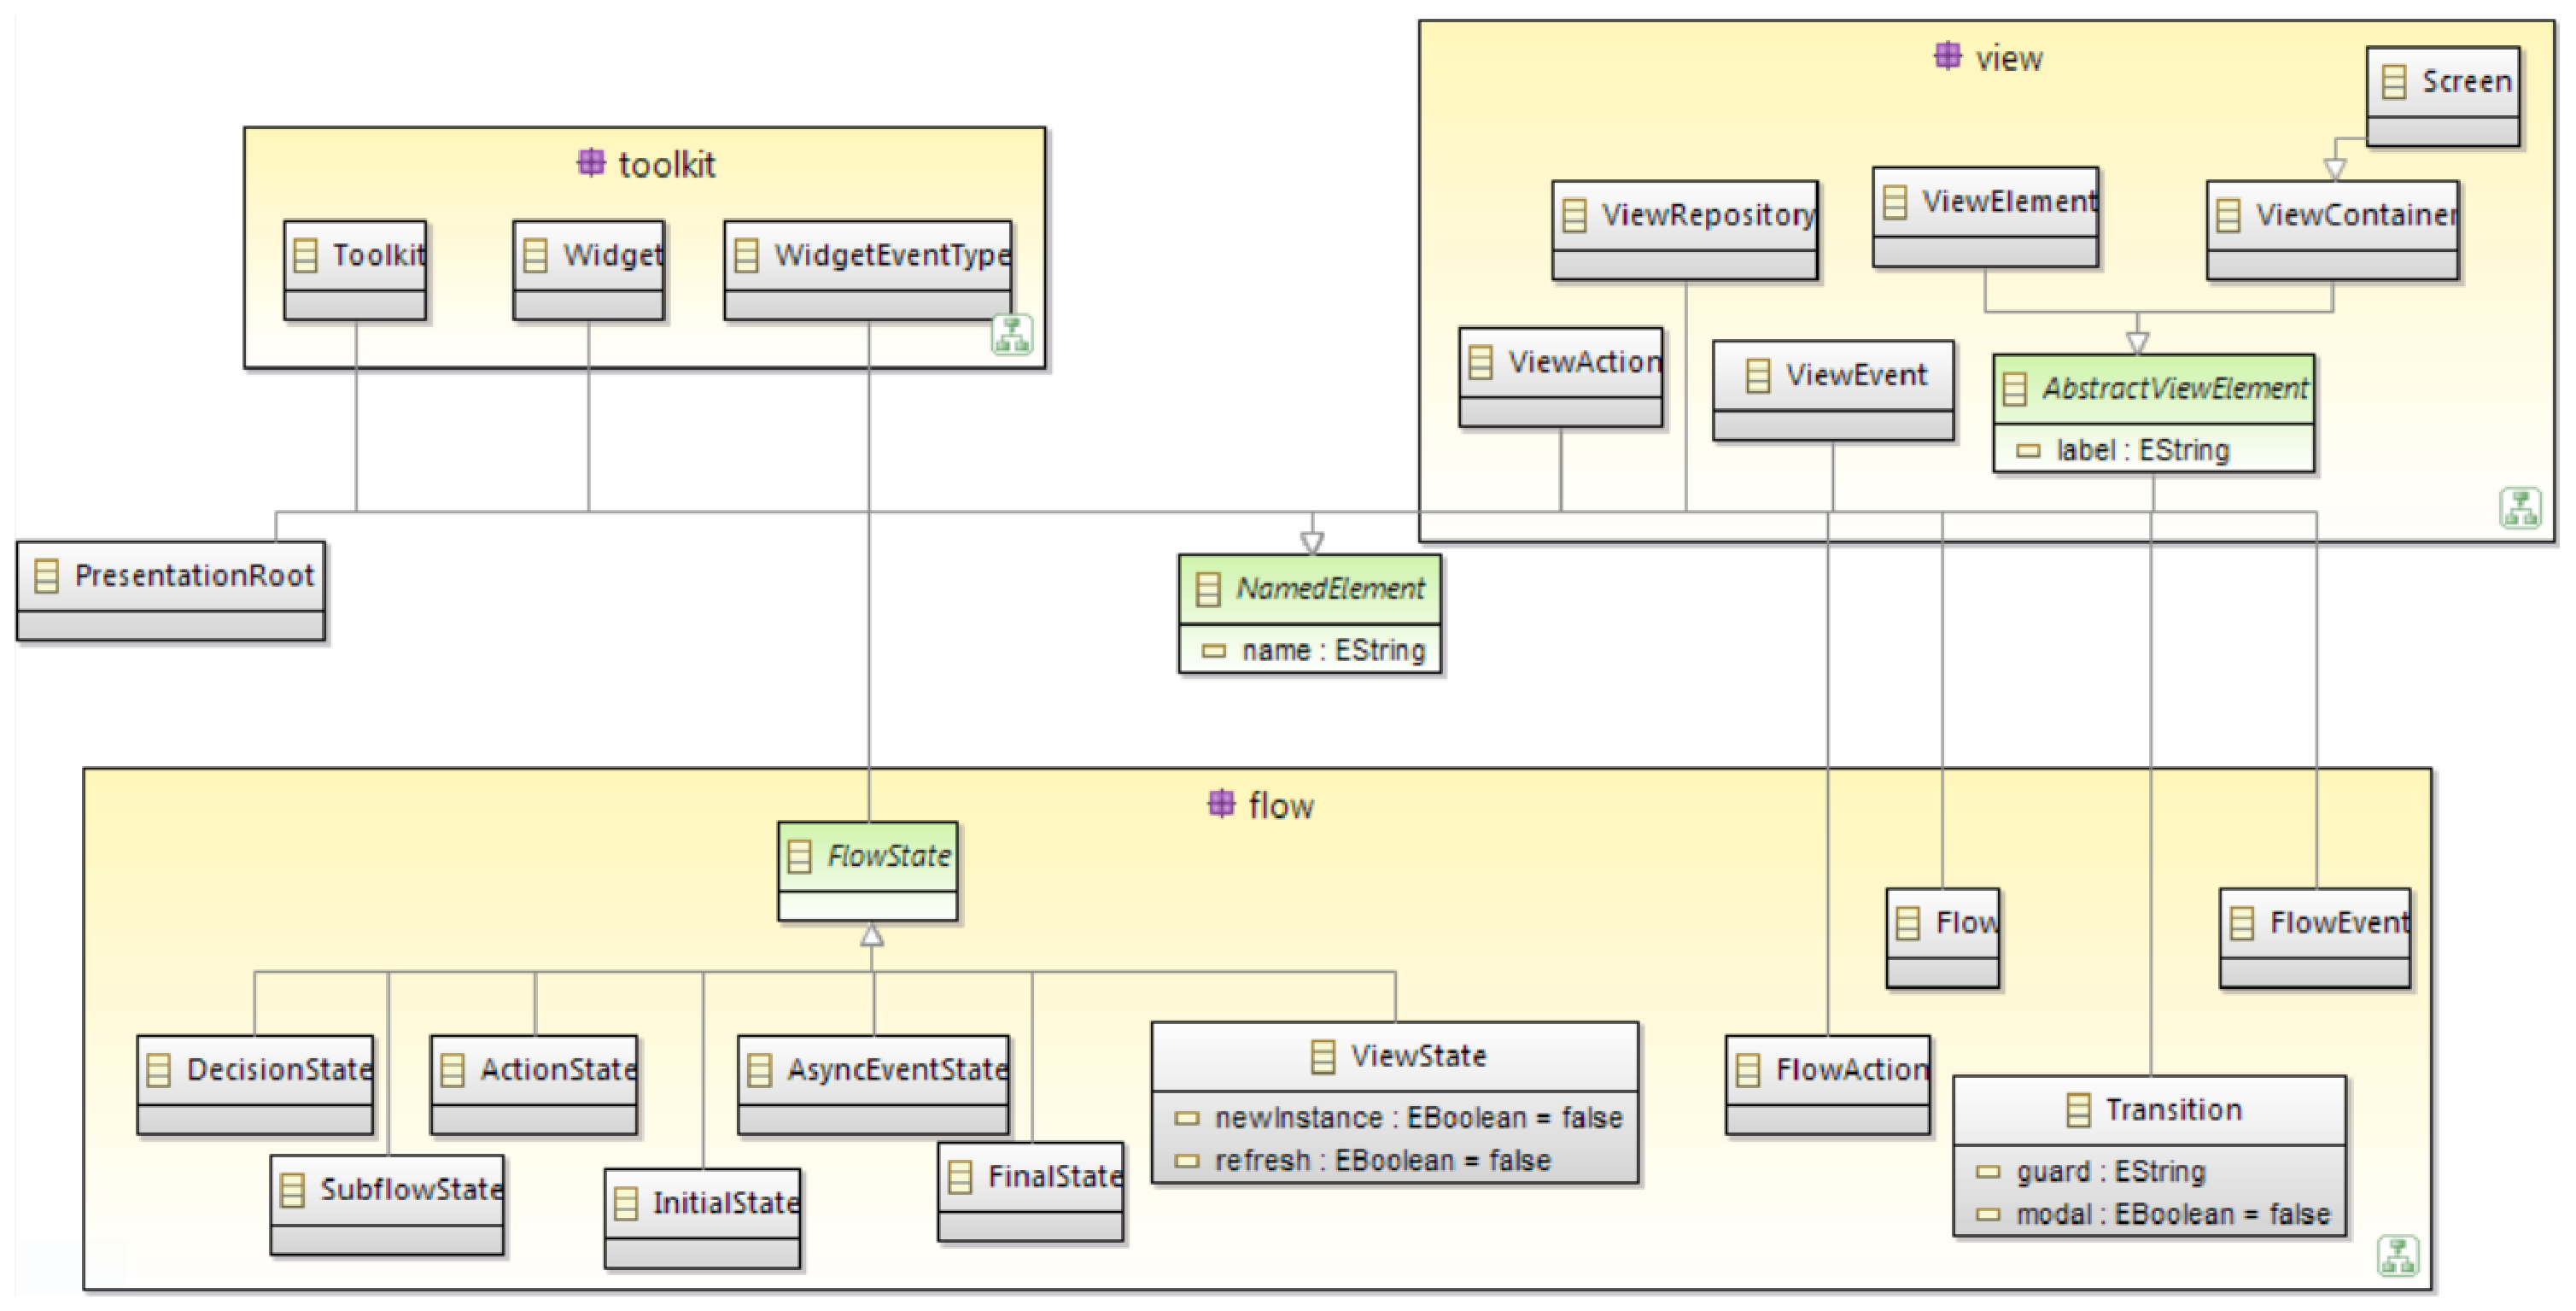
\includegraphics[scale=.24]{img/cinematic_m2.eps} 
  \ec{}

\end{slide}

% Le concept de Cinematic dans Play
\overlays{3}{%
  \begin{slide}{Travaux > Cinematic > Dans \textit{Play!}}

    \begin{itemstep}
    \itemg \textbf{View :} Forme des pages web
    \itemg \textbf{Controller :} Gestion de l'affichage des vues
    \itemg \textbf{Route :} Configuration des routes
    \end{itemstep}
    \bc{} 
      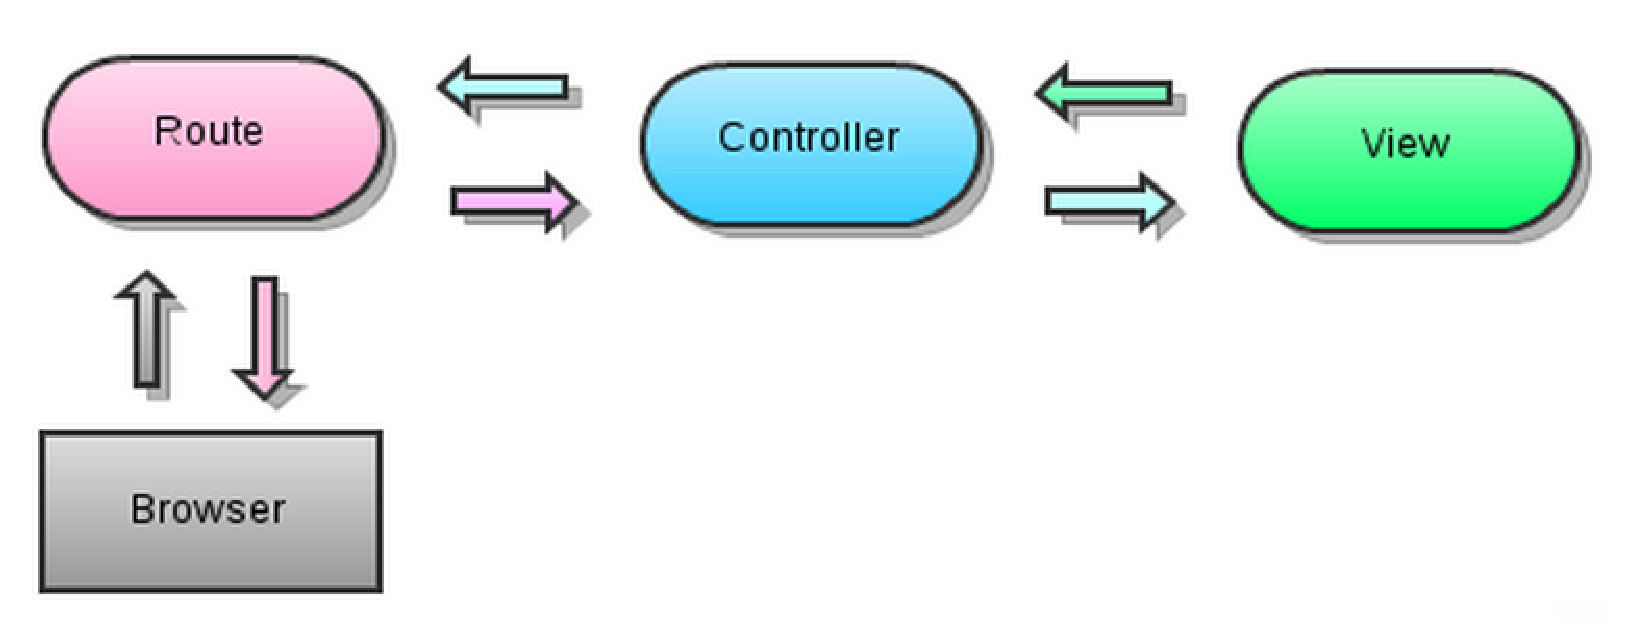
\includegraphics[scale=.3]{img/cinematic_play.eps} 
    \ec{}

  \end{slide}
}

% Concepts de Cinematic utilisés
\begin{slide}{Travaux > Cinematic > Concepts utilisés}

  \bc{} 
    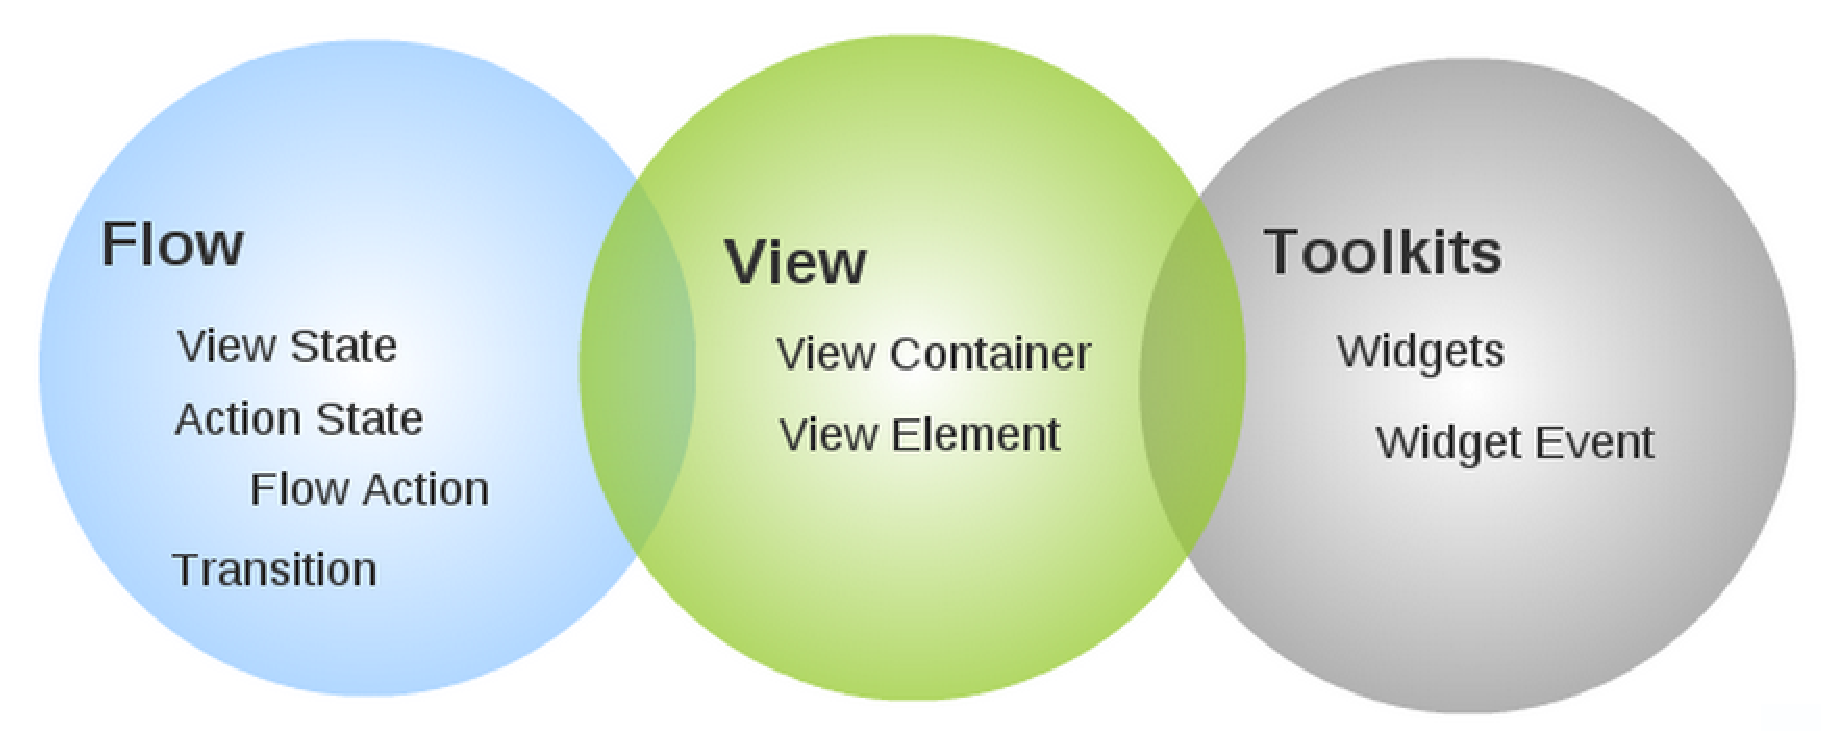
\includegraphics[scale=.3]{img/cinematic_concepts.eps} 
  \ec{}

\end{slide}

% A
\begin{slide}{Travaux > Cinematic > Scénario d'exemple}
  \bc{} 
    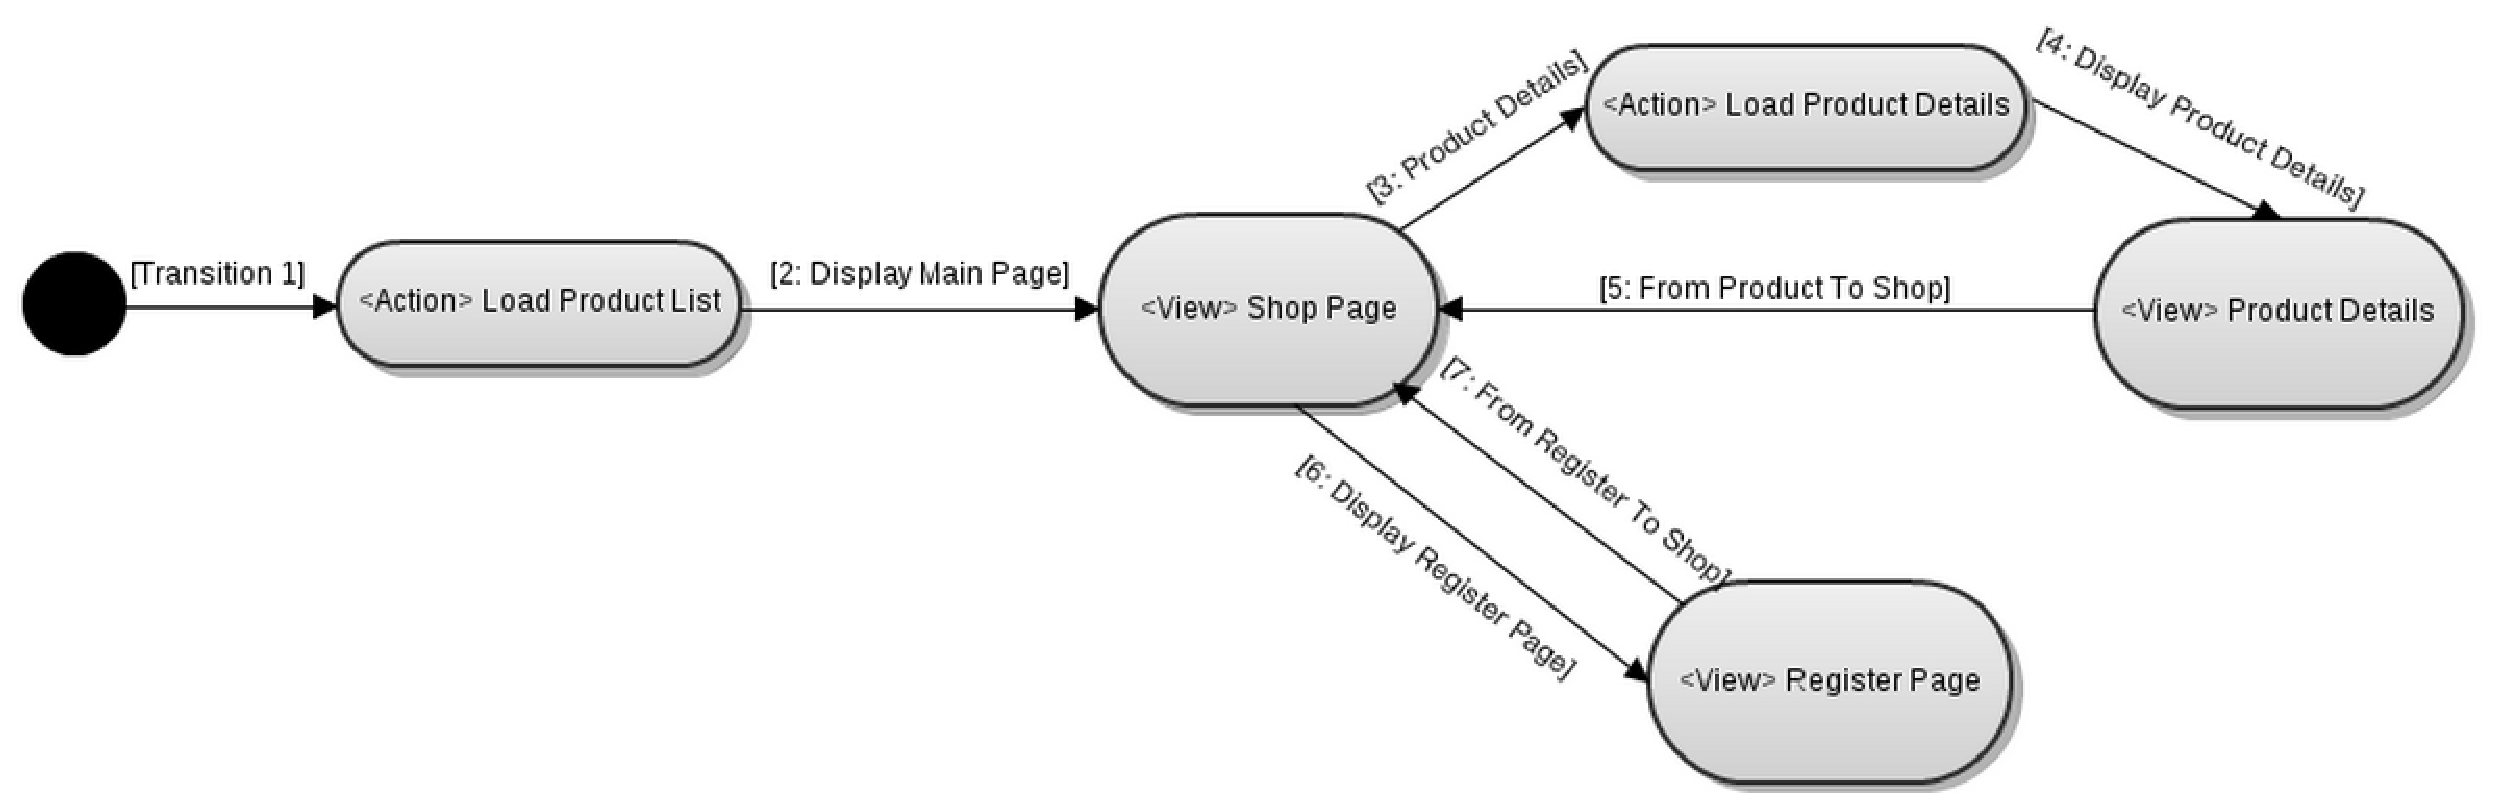
\includegraphics[scale=.25]{img/cinematic_act.eps} 
  \ec{}
\end{slide}

% B
\begin{slide}{Travaux > Cinematic > Générateur de code}
    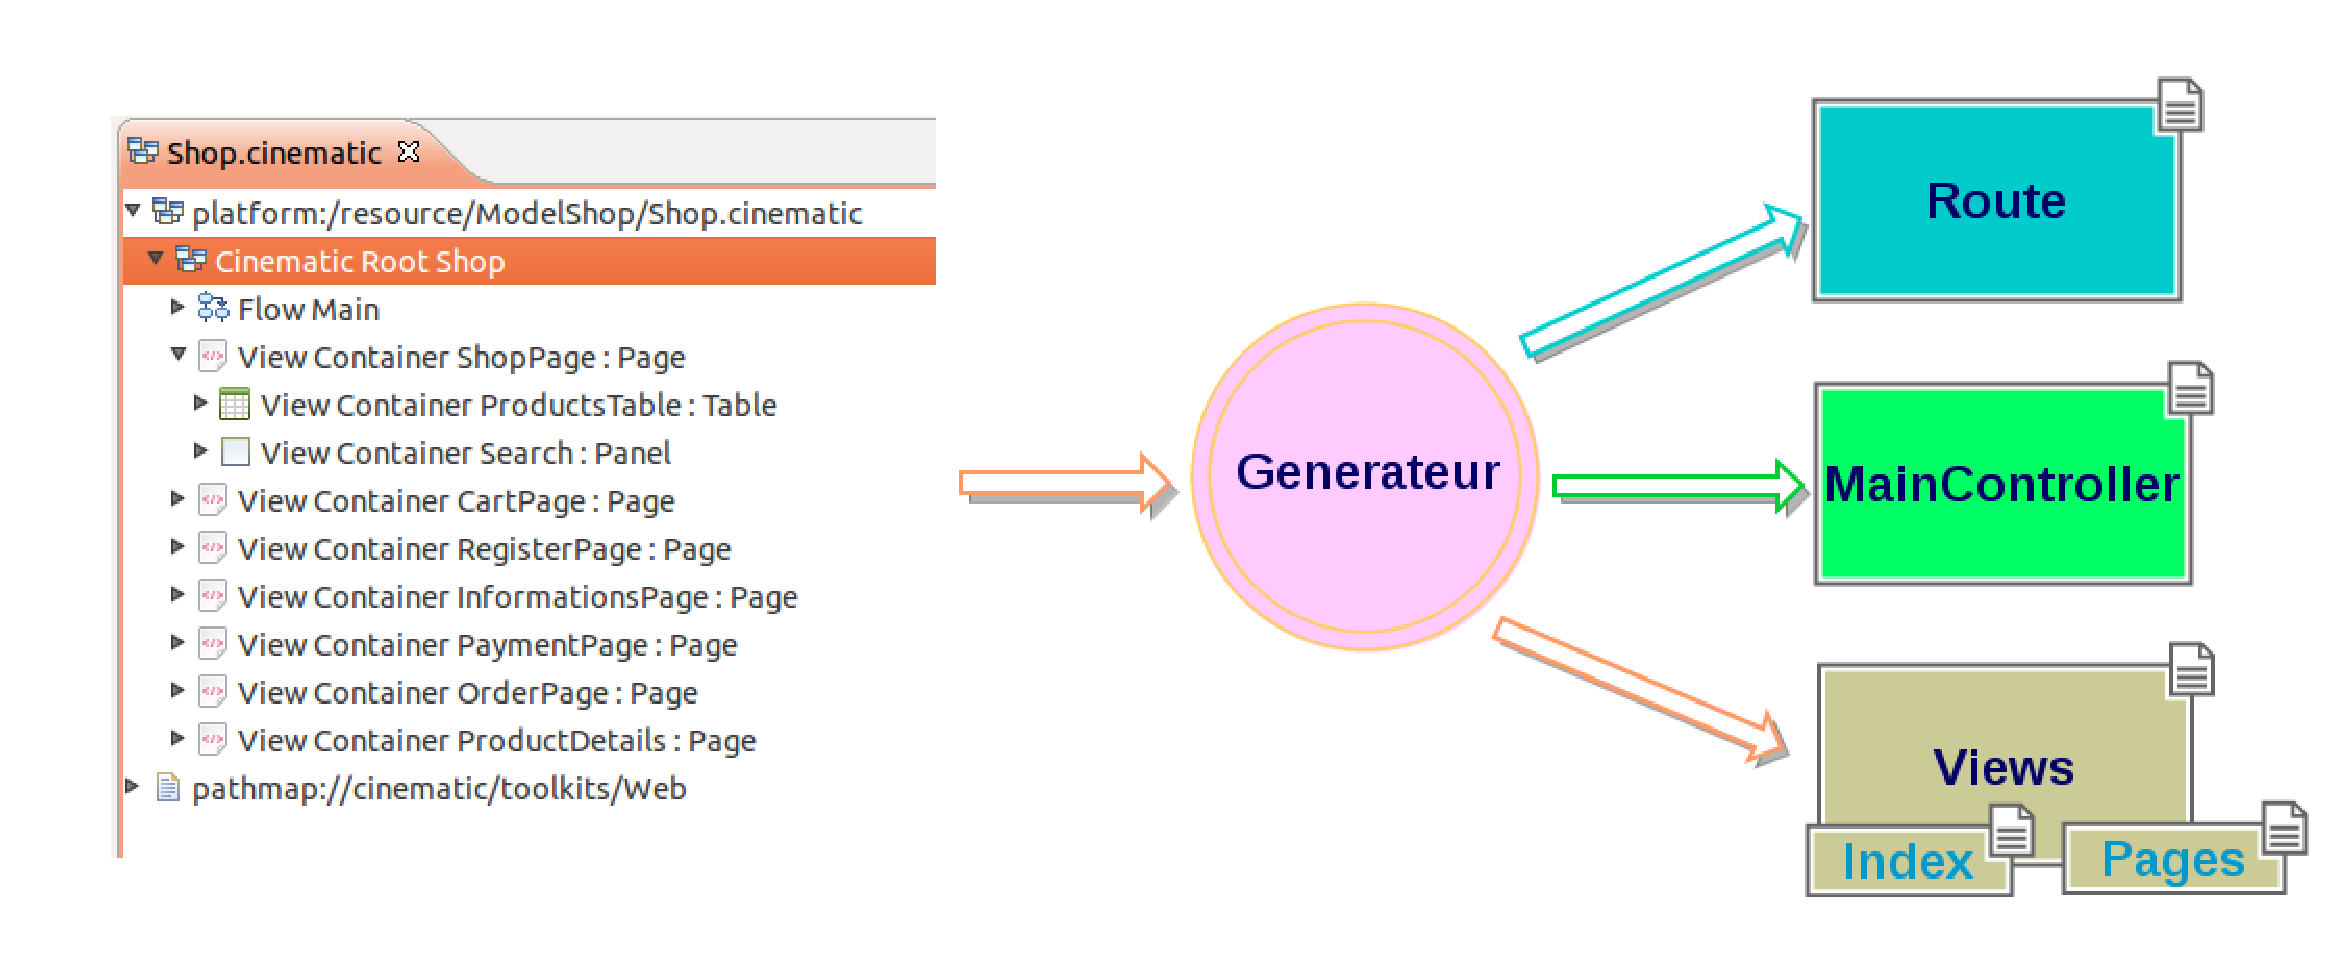
\includegraphics[scale=.3]{img/cinematic_gen.eps} 
\end{slide}

% B
\begin{slide}{Travaux > Cinematic > Générateur de code}
    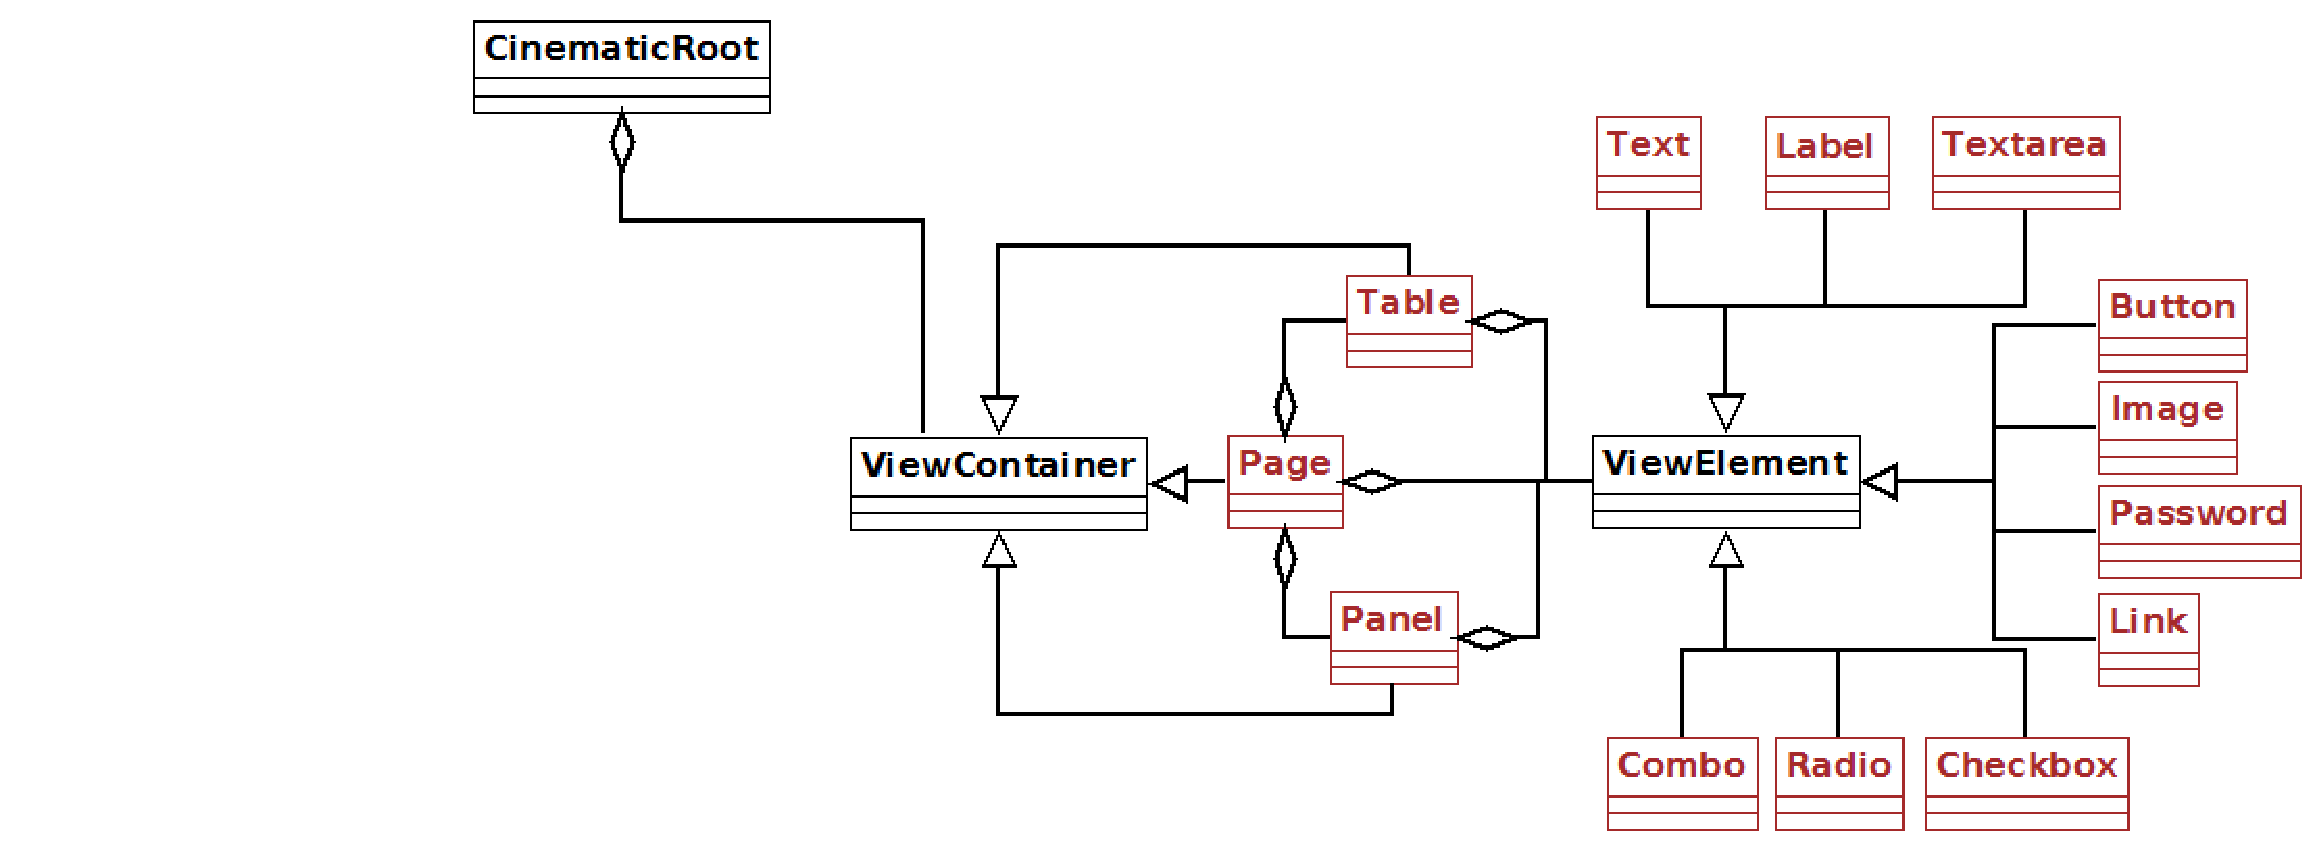
\includegraphics[scale=.3]{img/cinematic_exp1.eps} 
\end{slide}

% B
\begin{slide}{Travaux > Cinematic > Générateur de code}
    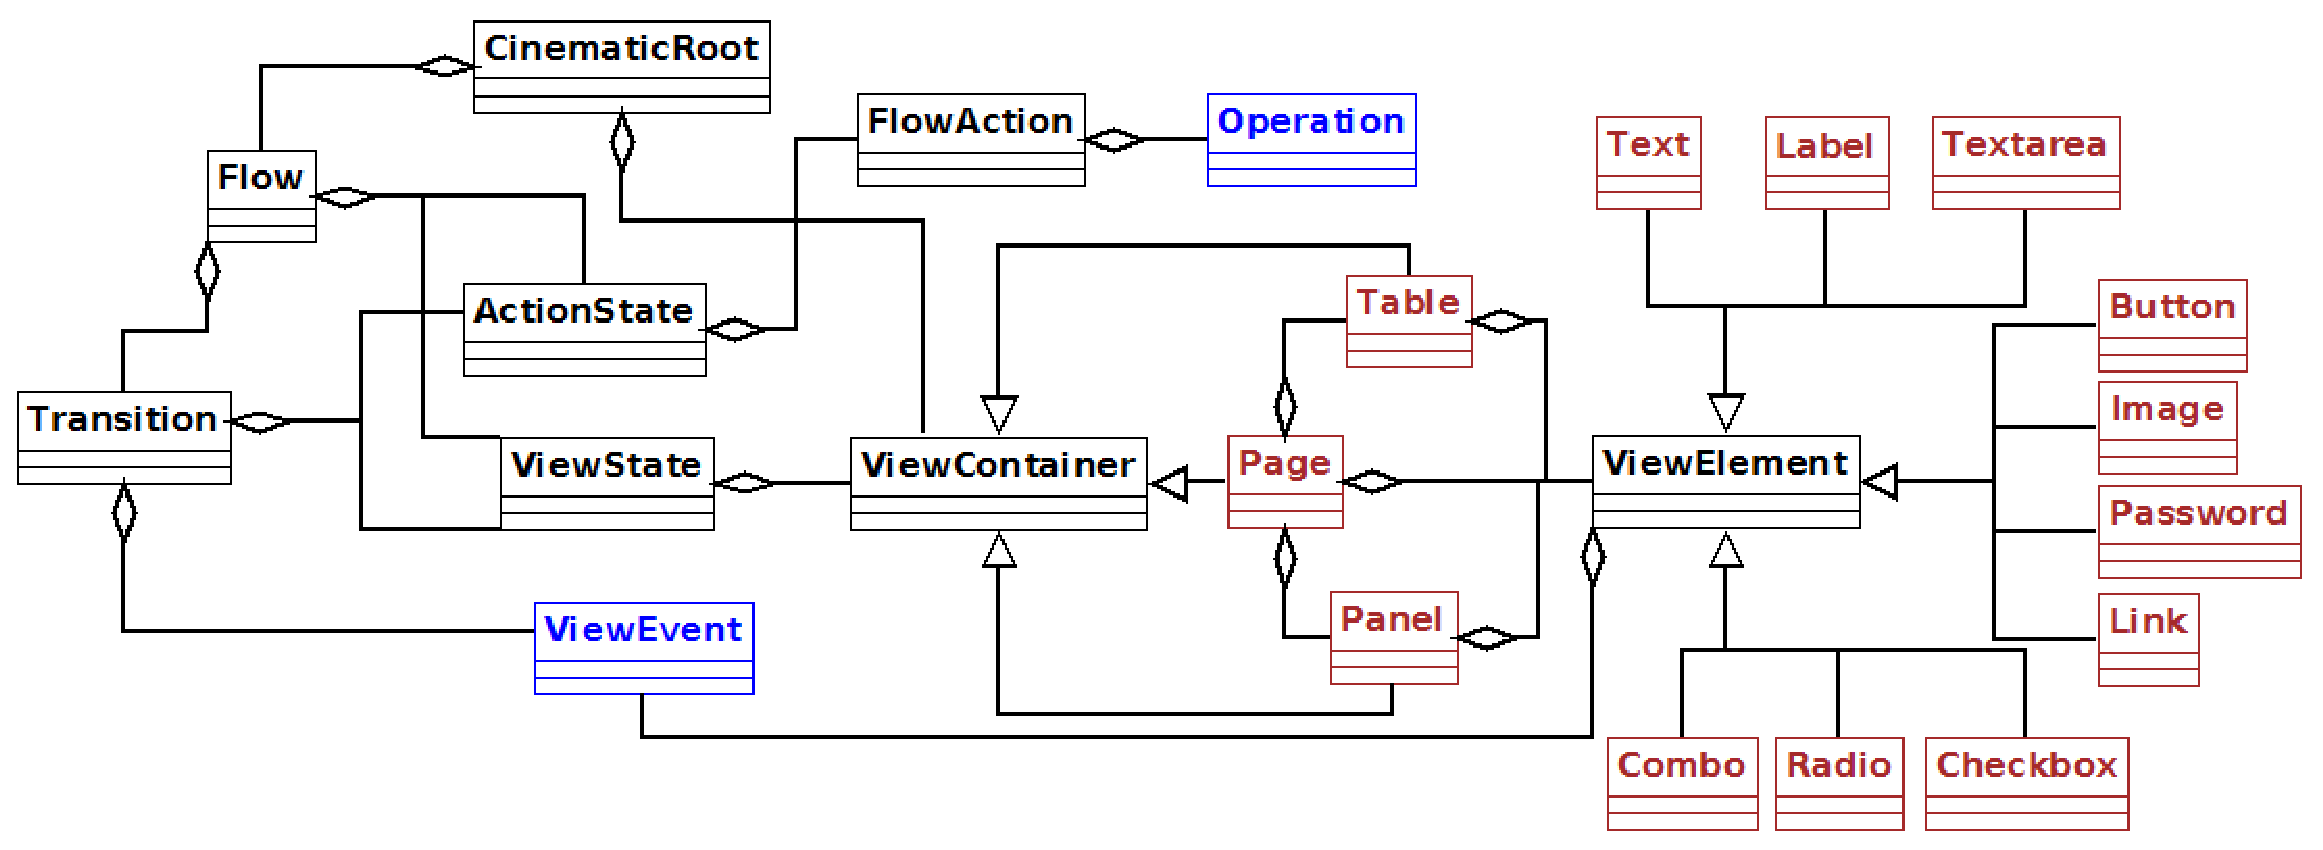
\includegraphics[scale=.3]{img/cinematic_exp2.eps} 
\end{slide}

% Deploiement
\begin{slide}[Box]{Deploiement}
  \bc{}
    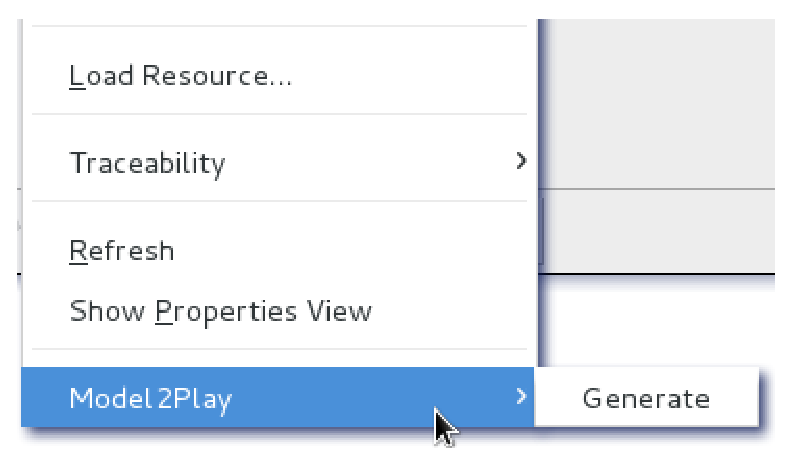
\includegraphics[scale=.4]{img/screen_menu.eps}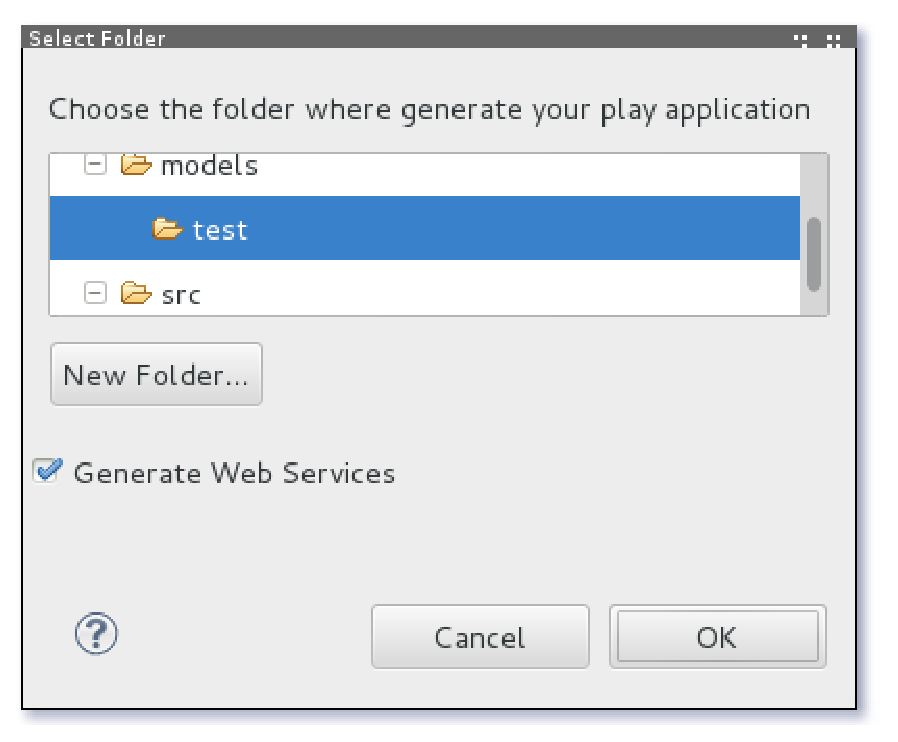
\includegraphics[scale=.35]{img/screen_ui.eps} 
  \ec{}
\end{slide}


% Bilan
\overlays{9}{%
\begin{slide}{Bilan}
    \bi
    \fromSlide{1}{\item[{\includegraphics[width=.4cm]{red-bullet-on-white}}]Contribution}
    \bi
    \fromSlide{2}{\item Génération d'application \textit{Play!} à partir de modèles Entity, SOA et Cinematic}
    \fromSlide{3}{\item Génération de Webservices}
    \ei
    \ei
    \vspace{.5cm}
    \bi
    \fromSlide{4}{\item[{\includegraphics[width=.4cm]{red-bullet-on-white}}]Problèmes persistants}
    \bi
    \fromSlide{5}{\item Fonctionalités des générateurs}
    \fromSlide{6}{\item Tests des générateurs}
    \ei
    \ei
    \vspace{.5cm}
    \bi
    \fromSlide{7}{\item[{\includegraphics[width=.4cm]{red-bullet-on-white}}]Bilan}
    \bi
    \fromSlide{8}{\item Acquisitions de nouvelles compétences}
    \fromSlide{9}{\item Travail collaboratif}
    \ei
    \ei
\end{slide}
}

% Questions
\begin{slide}{QUESTIONS ?}

\end{slide}


%%%%%%%%%%%%%%%%%%%%%%%%%%%%%%%%%%%%%%%%%%%%%%%%%%%%%%%%%%%%%%%%%%%%%%%%%%%%%%%%%%%%%%%%%%%%%%%
%% \overlays{7}{%
%%   \begin{slide}{Research topic}
%%     \fromSlide{1}{\textbf{Motivation :}}
%%     \bi
%%     \fromSlide{2}{\item[{\includegraphics[width=.4cm]{green-bullet-on-white}}] Software changes} % ya plein de logiciels faut les améliorer mais cest compliqué car dangereux toussa
%%     \fromSlide{3}{\item [{\includegraphics[width=.4cm]{green-bullet-on-white}}] Group actual knowledge} % cest bien de tout rassembler
%%     \fromSlide{4}{\item [{\includegraphics[width=.4cm]{green-bullet-on-white}}] Facilitate discussion and changes} % facilite les échanges entre scientifique et donc mieux prévoir les chgmt
%%     \ei
%%     \vspace{0,5cm}
%%     \fromSlide{5}{\textbf{How ?:}}
%%     \bi
%%     \fromSlide{6}{\item  Systematic review.} % cest quoi toussa cest bien pour la problematique
%%     \fromSlide{7}{
%%       \psovalbox*[fillcolor=yellow]%
%%                  {\parbox{7cm}{\begin{center}\parbox{9cm}{\hspace{-.5cm}
%%                          Software Architecture Change Characterization Scheme)}\end{center}}}}
%%     \ei
%%   \end{slide}
%% }
%% %%%%%%%%%%%%%%%%%%%%%%%%%%%%%%%%%%%%%%%%%%%%%%%%%%%%%%%%%%%%%%%%%%%%%%%%%%%%%    

%% \overlays{4}{%
%%   \begin{slide}{Main results 1/2}
%%     \vspace{-1cm}
%%     \textbf{Systematic review}
%%     \fromSlide{1}{\textbf{Method:}}
%%     \bi
%%     \fromSlide{2}{\item[{\includegraphics[width=.4cm]{green-bullet-on-white}}] Software changes} % ya plein de logiciels faut les améliorer mais cest compliqué car dangereux toussa
%%     \fromSlide{3}{\item [{\includegraphics[width=.4cm]{green-bullet-on-white}}] Group actual knowledge} % cest bien de tout rassembler
%%     \fromSlide{4}{\item [{\includegraphics[width=.4cm]{green-bullet-on-white}}] Facilitate discussion an changes} % facilite les échanges entre scientifique et donc mieux prévoir les chgmt
%%     \ei

%%   \end{slide}
%% }

%% %%%%%%%%%%%%%%%%%%%%%%%%%%%%%%%%%%%%%%%%%%%%%%%%%%%%%%%%%%%%%%%%%%%%%%%%%%%

%% \overlays{2}{%
%%   \begin{slide}{Main result 2/2}
%%     \vspace{-1cm}
%%     \textbf{Software Architecture Change Characterization Scheme :}
%%     \fromSlide{2}{
%%       \begin{figure}[t]
%%         \begin{center}
%%           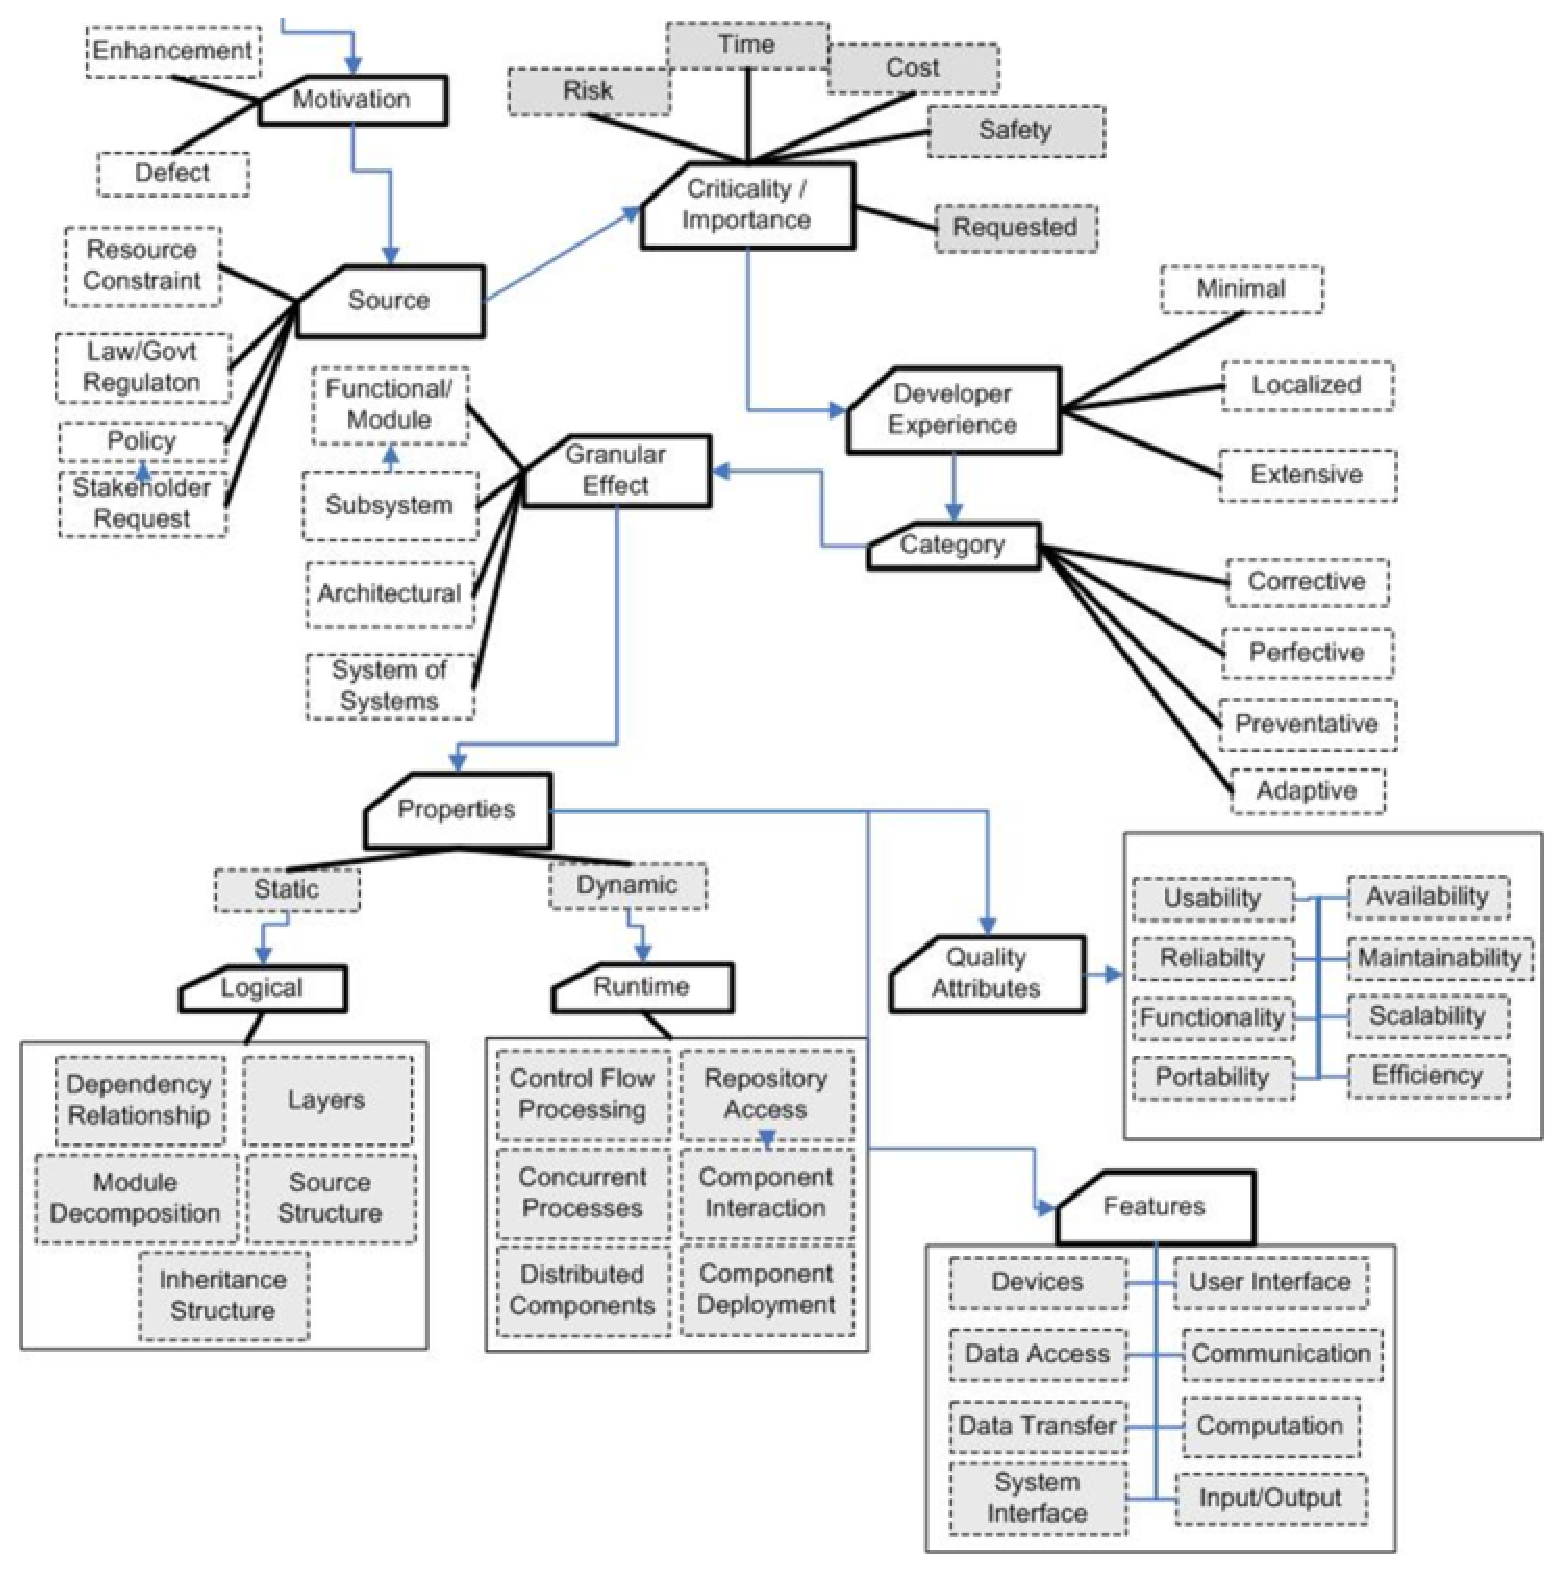
\includegraphics[width=0.72\textwidth]{img/saccs}
%%         \end{center}
%%       \end{figure}
%%     }
%%   \end{slide}
%% }


%% %%%%%%%%%%%%%%%%%%%%%%%%%%%%%%%%%%%%%%%%%%%%%%%%%%%%%%%%%%%%%%%%%%%%%%%%%%%
%% \overlays{8}{%
%%   \begin{slide}{Research topic's matter}
%%     %    \vspace{-1cm}
%%     \textbf{Main results}
%%     \bi
%%     \fromSlide{1}{\item[{\includegraphics[width=.4cm]{red-bullet-on-white}}]Contribution}
%%     \bi
%%     \fromSlide{2}{\item Systematic review of software change}
%%     \fromSlide{3}{\item Software Architecture Change Characterization Scheme}
%%     \ei
%%     \ei
%%     \vspace{1cm}
%%     \fromSlide{4}{\textbf{Consequences :}}
%%     \bi
%%     \fromSlide{5}{\item [{\includegraphics[width=.4cm]{red-bullet-on-white}}]  Relevant results}
%%     % resultat pertinant grace a la sytematic review
%%     \fromSlide{6}{\item SACCS's strengh} 
%%     %Conséquence de ce processus, outil de qualité
%%     \fromSlide{7}{\item A usefull tool for developers} 
%%     % aide les developers a prendes des décisions
%%     \fromSlide{8}{\item An inovation} 
%%     % le premier du genre 
%%     \ei  
%%   \end{slide}
%% }

%% %% %% %%%%%%%%%%%%%%%%%%%%%%%%%%%%%%%%%%%%%%%%%%%%%%%%%%%%%%%%%%%%%%%%%%%%%%
%% %% \overlays{3}{%
%% %%   \begin{slide}[Wipe]{Using Join Point Interfaces (JPI)}
%% %%     \vspace{-1cm}
%% %%     \textbf{Dépendencies}
%% %%     \vspace{1cm}
%% %%     \begin{figure}
%% %%       \centering
%% %%       \onlySlide*{2}{ \vspace{0,5cm}  \hfill  \includegraphics[scale=0.35]{img/diag3ab.eps}}
%% %%       \onlySlide*{3}{     \includegraphics[scale=0.35]{img/diag3b.eps}}
%% %%     \end{figure}
%% %%   \end{slide}
%% %% }
%% %% %%%%%%%%%%%%%%%%%%%%%%%%%%%%%%%%%%%%%%%%%%%%%%%%%%%%%%%%%%%%%%%%%%%%%%
%% %% \overlays{2}{%
%% %% \begin{slide}[Wipe]{Polymorphic join points}
%% %%   \vspace{-1cm}
%% %%   \textbf{Example}
%% %%   \vspace{1cm}
%% %%   \begin{figure}
%% %%     \centering
%% %%     \includegraphics[scale=0.35]{img/dispatch.eps}
%% %%   \end{figure}
%% %%   \vspace{1cm}
%% %%   \bi
%% %%   \item
%% %%     \textit{Dispatch}
%% %%   \item 
%% %%  \fromSlide{2}{   Manual ?}
%% %%   \ei
%% %% \end{slide}
%% %% }
%% %% %% %%%%%%%%%%%%%%%%%%%%%%%%%%%%%%%%%%%%%%%%%%%%%%%%%%%%%%%%%%%%%%%%%%%%%
%% %% %


%% %% %%%%%%%%%%%%%%%%%%%%%%%%%%%%%%%%%%%%%%%%%%%%%%%%%%%%%%%%%%%%%%%%%%%%%%


\end{document}
